One of the main differences between the conceptual mechanical design and the final design is the inclusion of 3D-printed harmonic gearboxes. The previous designs utilized a combination of standard spur gears and timing belts. It was determined that neither of these options provided the necessary precision without also introducing backlash into the system, which is nearly impossible to correct for with our feedback configuration. The solution was to design and implement a harmonic drive system. The harmonic gearbox locations are shown below in Figure \ref{fig:HarmonicGearboxLocations}

\begin{figure}[htp]
  \centering
  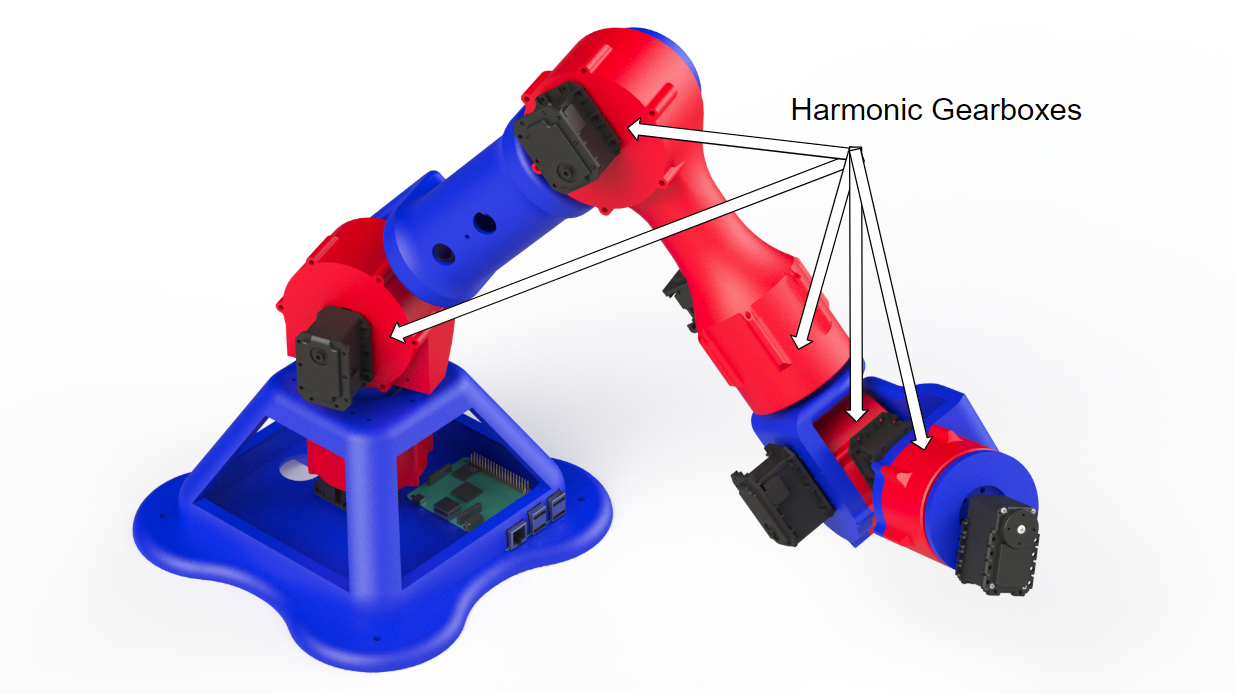
\includegraphics[width=.65\textwidth,frame]{HarmonicGearboxLocations}
  \caption{Harmonic Gearbox Locations}
  \label{fig:HarmonicGearboxLocations}
\end{figure}

As seen in Figure \ref{fig:HarmonicGearboxLocations}, each joint only requires a single actuator, which is a configuration not seen in the previous design. This is possible because harmonic drives allow for very high gear ratios with minimal backlash. The first prototype harmonic drive was provided by a posting on Thingiverse [citation]. This design was meant to be driven by a stepper motor and provided a gear ratio of 39:1. However, the gearboxes implemented in the manipulator need to be driven by a smart servo. Because the smart servo cannot drive as fast as a stepper motor, the ratio of 39:1 resulted in joint movement that was extremely slow. Additionally, given the link lengths and precision of the servos, only a gear ratio of 20:1 was necessary to meet the precision requirements of the system. For these reasons, a second harmonic drive was designed to provide the proper gear ratio of 20:1. Figure \ref{fig:ExplodedViewoftheHarmonicGearbox} provides an exploded view of the main structural components of the newest harmonic drive.

\begin{figure}[htp]
  \centering
  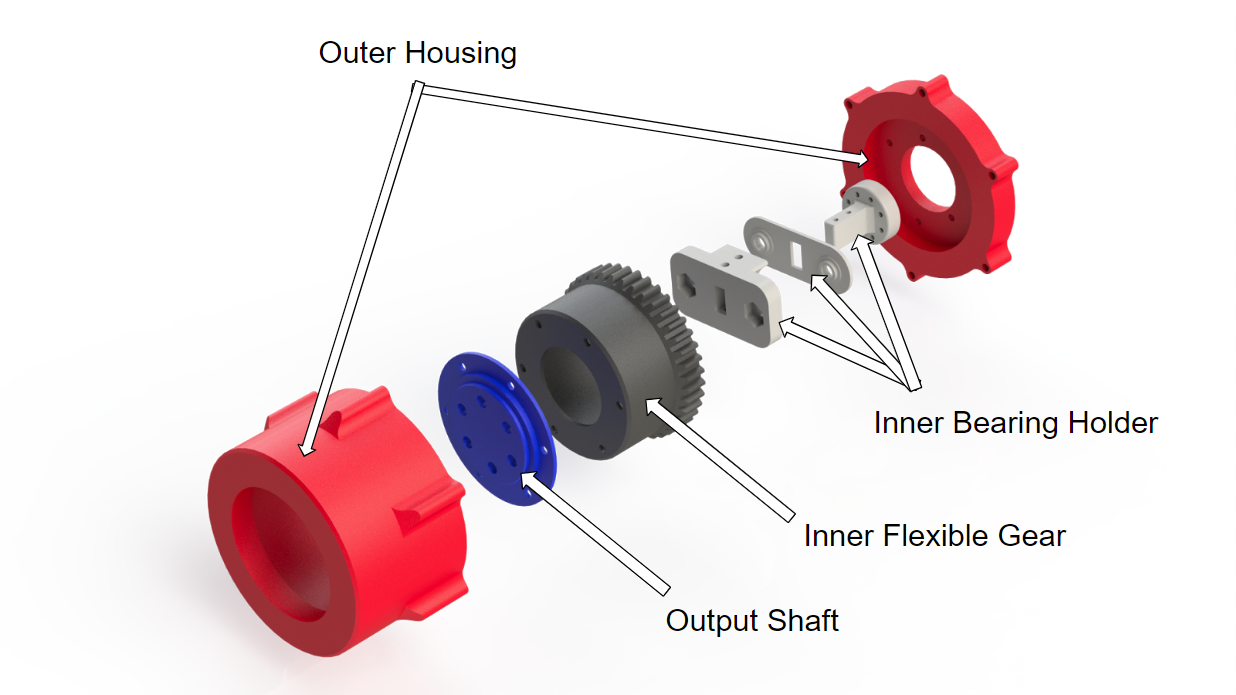
\includegraphics[width=.65\textwidth,frame]{ExplodedViewoftheHarmonicGearbox}
  \caption{Exploded View of the Harmonic Gearbox}
  \label{fig:ExplodedViewoftheHarmonicGearbox}
\end{figure}

As seen in Figure \ref{fig:ExplodedViewoftheHarmonicGearbox}, the basic harmonic drive design features an outer housing, a stiff output shaft, a flexible gear, and a bearing holder assembly. When fully assembled, the bearing holder sits on the inside of the flexible gear. As the servo drives the inner bearing holder, a continuous meshing of teeth occurs between the flexible gear and the set of teeth that are built into the outer housing. Because the inner set of teeth has two less teeth than the outer set (the inside has 40 while the outside has 42), the inner gear will move forward by two teeth per rotation of the bearing holder. This results in 1/20th of a rotation of the flexible gear per full rotation of the bearing holder. With the output shaft being attached to the flexible gear, the whole harmonic drive provides a ratio of 20:1.
